% !TEX encoding = UTF-8 Unicode
%!TEX root = ../Main/thesis.tex
% !TEX spellcheck = en-US
%%=========================================
\documentclass[../Main/thesis.tex]{subfiles}
\begin{document}
\chapter{Introduction}
\label{ch:introduction}
%The first chapter of a well-structured thesis is always an introduction, setting the scene with background, problem description, objectives, limitations, and then looking ahead to summarize what is in the rest of the report. 
%This is the part that readers look at first---\emph{so make sure it hooks them!}

%%=========================================
\section{Background}
\label{sec:background}
%In this section, you should present the problem that you are going to investigate or analyze; why this problem is of interest; what has, so far, been done to solve the problem, and which parts of the problem that remain.
%{\color{red}Below, I have set up some headings (subsection titles) without a number. 
%These are included to help you remember to cover the related issues. 
%The headings should be removed in your final print.}
%%=========================================
%\subsection*{Problem Formulation}
The associate press, a leading news organization, wrote: \say{Norwegian probe: Gearbox failure caused fatal 2016  crash}.
It was a news report of an airbus helicopter crash, on a small island outside of Bergen, the second largest city in Norway, cutting short the life of 13 people. The official cause of the crash: \say{A fatigue fracture in the main rotor gearbox.}. The anticipated question that arises after such catastrophic event is: was it preventable?
%The latter question has been the driving force of the development of methods and strategies, in order to mitigate such events.
\justify
%Since the industrial revolution, engines and machines have been the driving force for economic growth across industries such as automotive, airline, oil and gas, to name a few.
The latter question has been the driving force, behind the adoption of what is commonly known as predictive maintenance.
Since, machines are prone to failure, they must be monitored and maintained regularly, to avoid catastrophic breakdown.
The set of methods and strategies used to monitor, detect or predict onset of failure, and plan maintenance, are grouped under the umbrella term predictive maintenance.
\justify
%To mitigate equipment and machines proclivity toward failure and the associated cost, a process called predictive maintenance has been developed within the industrial community.

Formally, predictive maintenance  for machines and industrial equipment can be defined as a maintenance philosophy or more generally a framework, with a set of standards and methods, used to predict and prevent machine failure. This maintenance philosophy, when correctly implemented, increases machine life time, reduces downtime and maintenance cost. The aim here, is to detect as early as possible incipient failure and take appropriate actions.
\justify
Most industrial machines or equipment, rely on one or more rotating component(s) such as a gear box or a shaft. These rotating components,
are sometime coupled with bearings in order to facilitate their rotation.
In rotating machines, more than $40 \% $ of failure can be attributed to bearing faults (\cite{albrecht1986}), as shown in figure \ref{fig:pie}, which displays the distribution of faults in rotating machines. By facilitating rotation movements, bearings can be subjected to large load and mechanical forces, which can lead to slowly propagating defects. 
\justify
Most commonly applied methods in predictive maintenance for bearing fault detection rely on the Fourier transform.
Here is why: To monitor bearing for eventual failures, one or more sensors are used to record their vibrating movement periodically. Each record or sample is called a bearing vibration signal. Because of their geometry, bearings failures are associated to specifics frequencies call defect frequencies, derived from each bearing type geometrical properties. Furthermore, the core of bearings monitoring, rest on the identification of the failure frequencies and their secondary effects. This is accomplished by Fourier transforming a target vibration signal into its corresponding frequency spectrum, and searching for eventual failure frequencies. 

\begin{figure}[H] %  figure placement: here, top, bottom, or page
   \centering
   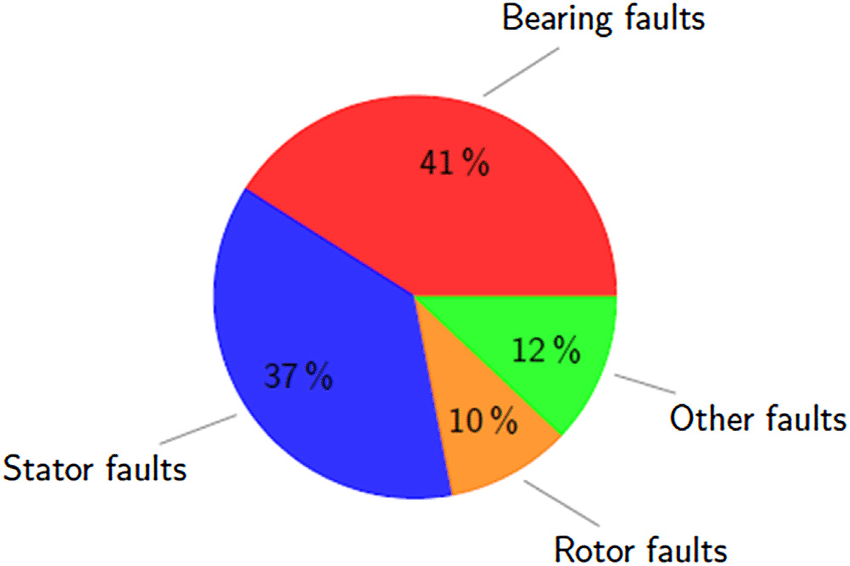
\includegraphics[width=4in]{../fig/pie.png} 
   \caption{Failure distribution in a rotating machine. }
   \label{fig:pie}
\end{figure}
\justify
Because a bearing vibration signal can be \say{contaminated} by other signals from different sources, most bearing fault detection methods apply a set of transformations to the target signal, before applying the Fourier transform. These \say{pre-processing} aim at isolating part of the signal that contained relevant diagnostic information. One of the most widely used method which accomplishes this with elegance, is the so call high frequency resonance technique (HFRT). Its apply a series of \say{filtering} operations in order to seep through, only part of the vibration signal, that contained potential traces of failure. The filtering operations, which are mathematical operations, are: high, low and band pass filtering. As their name indicate, a high pass filtering operation removes all low frequencies in a target signal, while a low pass filter accomplishes the apposite.
A band pass filter removes all frequencies bellow and above predefined thresholds. 
\justify
As will be shown later, a bearing with a defect, generates pulse like signals, buried deep inside the vibration signal, which can introduce non linearity as well as rendering the signal non stationary. Such pulses are temporal events, that the high frequency resonance technique (HFRT) attempts to isolate through filtering operations. However, the latter are not designed to resolve such phenomenon. Therefore, the spectrum derived from the HFRT can be noisy, making failure frequency detection challenging at times. In addition, the Fourier transform operates in the frequency domain, therefore can not properly resolve temporal events. Furthermore, the basis functions of the Fourier transform are trigonometric extensions that are not compactly supported. Recall that a compactly supported function on a closed interval, has non zero value within the interval and zero else where. This property allows capturing pule like signals, since a pulse is approximated as a compactly supported function.
To circumvent the aforementioned issues, this thesis presents an alternative method, based on Hilbert Huang transform (HHT), for bearing fault detection. By design, the Hilbert Huang transform can efficiently deal with signals that exhibit temporal features. Furthermore, in applying the Hilbert Huang transform, the goal is to resolve all temporal events before generating the frequency spectrum of a target vibration signal. This strategy not only expose any potential anomalies in the signal, caused by a bearing failure, its also generate a \say{clean}  frequency spectrum.


\justify
The Hilbert Huang transform was developed recently by  Huang, (\cite{huang98}) to deal efficiently with non linear and non stationary processes. It decomposes data adaptively 
into its sub-components by using the so called empirical mode decomposition (EMD). Unlike Fourier transform where trigonometric functions are used to decompose signals, adaptive decomposition means that 
the basis functions are completely determined by the data itself, (\cite{huang08}). This allow in theory, to access intrinsic and salient properties of data
\justify
In this brief introduction, the high frequency resonance technique (HFRT) was introduced as one of the prevalent methods used in bearing fault detection. Some of its weaknesses were  briefly outlined, and the Hilbert Huang transform (HHT) was introduced as a possible fix. To further understand the HFRT and the HHT, section \ref{sec:relatedwork} presents a literature survey, covering both methods while outlining their respective strengths and weaknesses.
To set apart the contribution of this thesis from what has been previously accomplished, section \ref{sec:contributions} describes in detailed the proposed method for bearing fault detection, based on Hilbert Huang transform.
\justify
In general, at the core of bearing fault detection are: the Fourier transform, signal filtering and the Hilbert transform, which was not mentioned so far. Therefore,
 Chapter \ref{sec:chapter2} gives a brief introduction of the Fourier analysis, outlines the Hilbert transform and presents the basics of signal filtering. Moreover, the high frequency resonance technique, which is the predominant method in bearing fault detection, is applied to a case study, in order to detect bearing failure frequencies. To show the contribution of this thesis, Chapter \ref{sec:hht}
gives a thorough presentation of the proposed method. It covers the Hilbert Huang transform, describes in detailed the application of Hilbert Huang transform to bearing fault detection, and uses a case study to demonstrate the efficiency of this method. 
To conclude this thesis, Chapter \ref{sec:conclusions} sum up what has been done, outline some of its weaknesses and gives a road map on how to improve up on them.
%The detailed treatment of these methods and the 
%%=========================================
\clearpage
\section{Literature review}
\label{sec:relatedwork}
As part of nearly all rotating machines, rolling bearing elements are one of the most frequent reasons for machine breakdown (\cite{randal2010}). A rolling bearing element is made of mainly four parts, which are shown in Figure \ref{fig:bearing-s}: The outer race indicated by 1, the balls trapped in the cage and labeled by 2 and 3 respectively. Finally, the inner race identified by 4 and 5. To facilitate machine rotation, a rotating shaft, which is a long cylindrical tube, is placed within the inner ring.
\begin{figure}[H]
	\centering
	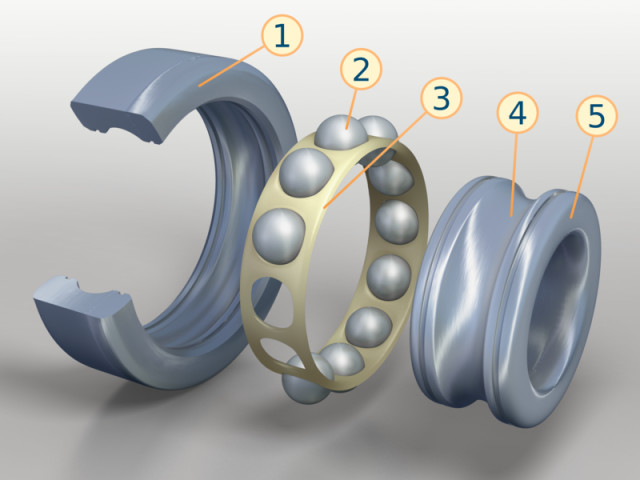
\includegraphics[width=0.5\linewidth]{../fig/bearing-s}
	\caption{Exploded view of a rolling bearing. 1: outer race or ring, 2: balls or roller elements, 3: cage, 4 and 5: inner race or ring.}
	\label{fig:bearing-s}
\end{figure}
\justify
Premature and unexpected bearing breakdown, can halt production and incur high cost. In the worst case scenario, human lives can be impacted. To avert dramatic consequences of bearing failure, it is therefore crucial to detect incipient faults and take appropriate actions.
\justify
The geometry of a bearing is important in understanding its dynamic, and detecting early sign of failure.
 A key fact in bearing fault detection, is that a failure can be detected at a given frequency, called characteristic defect frequency or failure frequency. Here is why. A defect in one surface of a rolling element bearing also called balls, generates an impulse as it hits an other surface, (\cite{mcfadden1984a}, \cite{mcfadden1984b}). As the bearing rotates, the impulses will occur periodically with a frequency (the defect frequency) which is uniquely determined by the location of the defect (\cite{mcfadden1984a}). Consequently, the failure frequency is derived from the bearing physical characteristics, and the rotational speed of the machine housing the bearing, (\cite{mcfadden1984a}). Therefore, finding the failure frequencies is the basis for bearing fault detection in most cases.
%and can be found in the vibration signal frequency spectrum it generates. 
%The latter is obtained by transforming the vibration signal with a mathematical transformation such as Fourier transform. 
\justify
There are typically four failure frequencies: ball pass frequency outer race (BPFO), which is the frequency at which a defect strikes the outer ring. Similarly, the ball pass frequency inner race (BPFI) is the frequency at which a defect hits the inner race. The fundamental train frequency cage (FTF) and the ball spin frequency (BSF) are frequencies at which a fault tricks the cage and the rollers (balls), respectively.
\justify
Finding the failure frequencies entails, transforming the bearing vibration signal into its corresponding frequency spectrum, where the defect frequencies reside. However, this apparent simple task is challenging. The vibration signal of a bearing is \say{infected} by the signals of other machines components or other vibration sources (\cite{zhao2014}, \cite{mcfadden1984a}). In addition, at the onset of failure, the fault frequencies are very weak (\cite{zhao2014}). To efficiently detect failure frequencies, a de-noising of the signal is necessary and the weak early defect frequencies must be enhanced (\cite{zhao2014}). 
\justify
To address the aforementioned issues, several signal processing techniques have been proposed. The most prevalent are (\cite{zhao2014}): the high frequency resonance technique (HFRT) (\cite{darlow1974}), Spectral kurtosis (\cite{antoni2006a}, \cite{antoni2006b}, \cite{antoni2007}), wavelet analysis (\cite{lin2000}, \cite{qiu2006}), Hilbert Huang transform and the empirical mode decomposition (\cite{yu2005}, \cite{lei2011}), cyclostationary approach (\cite{antoni2004}, \cite{borghesani2013}, \cite{girondin2013}), minimum entropy deconvolution (\cite{sawalhi2007}, \cite{jiang2013} ), and stochastic resonance (\cite{tan2009}, \cite{he2012}). The most widely used method is however the high resonance frequency technique, because it is able to efficiently extract bearing diagnostic information, trough a sequence of filtering operations (\cite{zhao2014}).
%In addition, under harsh conditions such as time varying machine rotational speed and load or large shock, the vibration signals are low signal noise ration and non stationary \cite{zhao2014}.

\justify
One of the first work on bearing fault detection was by (\cite{balderston1969}), who investigated bearings rings and roller elements (balls) natural frequencies, and observed that the signal induced by bearings defects are located in the high frequency zone of resonance exited by the internal impact of the faults, (\cite{randal2010}). Let elaborate on this. As previously mention, a bearing defect will generate periodic impulses, which are forces that strike the bearing at the location of the defect, at a given frequency (failure frequency). When the failure frequency is equal, or nearly equal to the natural frequency of the bearing, this cause the latter to vibrate at a higher amplitude and frequency (\cite{mcfadden1984a}), then it would have at a different frequency. This phenomenon is called mechanical resonance. The latter will also occur in the machine housing the bearing, and in a potential sensor mounted on the bearing for collecting vibration data, (\cite{mcfadden1984a}).
\justify
 It is therefore critical to detect, and isolate the resonance exited by the impulses generated by bearing defects, which in theory can be visible in the bearing vibration signal. However, bearing diagnostic information in the form of failure frequencies are  difficult to be directly observable in the raw signal (\cite{randal2010}). This is due to the fact that the energy generated by the impulses induced by faults, are widely distributed over a wide range of frequencies (\cite{randal2010}).
 \justify
 To circumvent the latter difficulty, the high frequency resonance technique (HFRT) was developed and  allowed early detection of bearing failure (\cite{broderick1972}, \cite{burchill1973}, \cite{burchill1973b}, \cite{darlow1974}, \cite{darlow1975}, \cite{darlow1975b}, \cite{board1975},  \cite{randal2010}, \cite{gupta2016}, \cite{khadersab2018}).
In the high frequency resonance technique, a bearing vibration signal is  band pass filtered, envelop-detected, low pass filtered and finally decomposed into its frequency spectrum by the Fourier transform.
\justify
 The resonance induced by defects, are responses of the bearing, the machine housing the bearing, and possibly other surrounding machines (\cite{mcfadden1984a}). Therefore band pass filtering allows only the bearing signal to be recovered.
 The envelop detection procedure, extracts the high frequency resonance signal produced by the bearing defects. This signal is the superposition of two components: the high frequency resonance component and the low frequency bearing failure component. The latter is recovered by a low pass filter. 
 \justify
  Recall that a band pass filtering process in signal processing, filters a signal by only letting through desire frequencies. On the other hand, the envelop detection process, takes a target signal and returns its envelope. The latter is the curve formed by joining all peaks in the signal. In practice, the envelope signal is derived by taking the Hilbert transform of the band pass filtered signal. The low pass filter procedure, sips out low frequency components of a signal.
\justify
The diagnostic power of the high frequency resonance technique rests on the key fact that it uses the envelope of the band passed raw vibration signal, before performing the Fourier transform (\cite{mcfadden1984a}, \cite{randal2010}). The envelope signal contains nearly all the information generated by bearing faults. It is worth noting that the rollers elements located in the bearing cage are subjected to random slip, (\cite{mcfadden1984a}), and the bearing failure frequencies variation is of the order of 1-2$\%$ (\cite{randal2010}). This random slip changes the characteristics of the raw vibration signal, which makes it difficult to extract useful diagnostic information directly from the vibration raw signal, (\cite{randal2010}). However, the sequence of operation applied to the raw signal to obtain the envelope addresses specifically this situation of slip  (\cite{randal2010}). 
\justify
The envelope signal obtained from the High frequency resonance technique was also leveraged in other methods for bearing fault detection. For example, the spectral kurtosis method, uses the frequency spectrum of the envelope signal from the short time Fourier transform (STFT), to find the frequency band of the pulses generated by bearing fault (\cite{randal2010}). The spectral kurtosis uses fourth order statistical moment, to decompose the power of a signal with respect to frequencies, (\cite{randal2010}). Note that the short time Fourier transform uses fixed window size where the Fourier transform is applied. Akin to the spectral kurtosis, is the power spectral density (PSD) method, which uses second order statistics, to obtain the energy contribution of frequencies. The bearing failure frequency will generally produce a larger energy distribution.
% The random slip induce a fundamental change in the raw signal rendering it stochastic and makes it inefficient for bearing fault detection, \cite{randal2010}. 
\justify
 Although powerful, the high frequency resonance technique can produce a noisy spectrum for inner race or rolling element defect (\cite{mcfadden1984a}). The spectrum can become even more noisy when bearing defects are extensive (\cite{mcfadden1984a}). The dependency of the failure frequency on the machine rotation speed, can also be an issue as the rotating speed changes continuously or is unknown. Time varying rotation speed and load can cause the vibration signal to be non-stationary (\cite{zhao2014}), which makes the Fourier transform inadequate (\cite{huang98}, \cite{huang08}).
 \justify
  In addition, the Fourier transform uses trigonometric basis functions, that are not locally compact, and can not handle efficiently nonlinear and non-stationary signal (\cite{huang98}). The reader might argue that the short time Fourier transform, can handle non-stationary signal. However, the issue in this case is the selection of the window size. An other important issue for all frequency based method so far mentioned, are the selection of a resonance frequency band for band pass filtering the raw vibration signal (\cite{zhao2014}). The resonance frequency band, is the frequency band within which, the frequencies of resonance induced by the faults are located.
 \justify
 
 
\justify
 To extend bearing fault detection to cases where a Fourier transform based method or more generally frequency based methods are limited,
numerous contributions have been made towards alternative methods such as Hilbert Huang transform, wavelet transform and machine learning (\cite{zhang2019}, \cite{xiaoan2018}, \cite{rai2016}, \cite{konar2011}, \cite{rai2006} ). These methods can directly operate in the time domain (on the time signal), as opposed to Fourier transform based methods that require a frequency spectrum. 
\justify
The Hilbert Huang transform (HHT) as most signal analysis tool, is predicated on the key assumption that a signal has multiple components, and can be decomposed into single oscillatory modes called intrinsic mode functions (IMFs) (\cite{fosso2019}, \cite{huang08}, \cite{huang98}). It was developed to deal efficiently with nonlinear and non-stationary signals. As opposed to Fourier transfrom, the HHT method does not use a-priori basis functions. It uses local properties of a signal such as the extrema of a signal, the mean, with a series of operations to obtain a hierarchy of single component signals, that range from high to low frequency time signals. By using local properties, the HHT is able to model local events such as pulses emitted by bearing faults (which will be shown in this thesis). The wavelet transform on the other hand, utilizes locally compact basis functions, and was primarily used in geophysics, to model high frequency short duration seismic pulses, (\cite{albert09}), similar to those emitted by bearing faults .
\justify
For bearing fault detection, (\cite{fan2016}) decomposed the vibration signal obtained from a motor into intrinsic mode functions, and evaluated the Hilbert Huang energy spectrum (also called marginal spectrum) of each IMF, to detect sign of fatigue, oxidation and mechanical structure deformation. In the same fashion (\cite{peng2004}, \cite{soualhi2015}, \cite{osman2014},\cite{osman2013a}, \cite{osman2013b}, \cite{li2008}) Applied the marginal spectrum to identify bearing characteristic defect frequencies. The energy spectrum also called power spectrum or energy density, is the energy contribution of each frequency, derived from the intrinsic mode functions.
To compute the energy density, the Hilbert transform of the absolute value of the square of an IMF is first computed. Secondly, the integral of the latter is evaluated over the domain of variability of the signal. The Hilbert transform of a signal is the convolution of the signal with the function $\frac{1}{\pi t}$, where $t$ is a dummy variable.
\justify
One of the issue of the Hilbert Huang transform, is selecting the appropriate intrinsic mode functions (\cite{fosso2019}). The IMFs obtained from a target signal, are hierarchy of mono component signals, ranging from high to low frequency. However, due to a phenomenon called mode mixing, an IMF, rather then having a single oscillatory mode, can have more than one mode, resulting an IMF to lose its physical meaning (\cite{fosso2019}). For a given process such as the vibration of a bearing in a motor, there exists multiple sub processes corresponding to the vibration of sub components of the motor and the bearing. Therefore mapping the correct IMFs to the corresponding sub processes is a daunting task.
\justify
 To resolve this issue, (\cite{osman2013a}, \cite{osman2013b} ) used a linear combination of two similarities measure (Linear and non-linear similarity) to select the target IMF and applied the energy spectrum of the IMFs to identify bearing failure frequencies. The similarities measures, quantifies the \say{sameness} of two distributions.
In the same fashion (\cite{osman2014}) applied a weighted D'Agostino Pearson (DP) normality test to select the more relevant IMFs (IMF representing defect component). The DP test uses both the skewness and the kurtosis to assess normality.
The skewness is a statistical estimator that measures the symmetry of a probability distribution, while the kurtosis also a statistical estimator, measures the \say{tailedness} of a distribution. The Kurtosis and skewness of a normal distribution are 3 and 0 respectively. (\cite{peng2004}), used the correlation coefficient as a criteria for IMF selection.
\justify
A large majority of Hilbert Huang transform methods applied to bearing fault detection uses the energy spectrum of the IMFs to identify the bearing failure frequencies (more citation here)
\justify
 




%%=========================================

\section{Contributions }
\label{sec:contributions}
The ubiquity of Fourier transform in science and technology, is the proof of its efficiency in solving complex scientific and industrial problems, such as bearing fault detection. In the latter, Fourier transform is the core of several methods that rely on frequencies spectrum to identify bearing failure frequencies. One of the predominant methods is the so call high frequency resonance technique (HFRT). As outlined earlier, the high frequency resonance technique, first uses successive filtering operations to remove \say{noisy signals} in a target vibration signal, then apply Fourier transform. This result in a frequency spectrum, which may potentially contain a bearing failure frequency.
\justify
in spite of its wide spread application, the Fourier transform is not without \say{limitations}. The latter are the results of the mathematical assumptions imposed, in order to formulate a rigorous theoretical framework. One such assumption, is to say that a target signal is the superposition of trigonometrical extensions, each with constant amplitude and frequency.
This makes it hard to apply the Fourier transform to amplitude and frequency modulated signals, generated for example by changing load. In addition, Fourier transform operates in the frequency domain, thus unable to access temporal phenomenon in a signal. Lastly, applying the Fourier transform to a signal can produce a noisy frequency spectrum when bearing faults become pronounced. This can introduce challenges in the process of identifying bearing failure frequencies.  
\justify
To address the aforementioned issues, when it comes to bearing fault detection, this thesis introduces a mixed method. It comprises the Hilbert Huang transform coupled with a robust seasonal trend decomposition method, for bearing faults detection. There are three steps in this method: In step 1, the Hilbert Huang transform (HHT) is used to decompose a signal into nearly mono component signals. This is akin to the Fourier transform, except that there is no predefined basis functions, and the resulting components reside in the time domain. In step 2, the seasonal parts of each component are extracted though the so called seasonal trend decomposition by LOESS method (STL). The seasonal parts are the oscillatory components. In the last step, the power spectrum density of each oscillatory part is computed through the periodogram which is an estimation of the power spectrum density. The latter is the energy distribution of the frequency spectrum. The power spectrum, essentially shows the energy contribution of each frequency component of a signal.
\justify
The difference between our methods and the HFRT is that we obtained a clear, noiseless spectrum, compared to the HRFT method whose spectrum can be noisy. This allows for an easy detection of bearing failure frequency.

%%=========================================

\blankpage
\end{document}
